
\section{Zenodo's dataset}
\subsection{Description of the dataset}
The scripts used in the last thesis were taken and applied to the new Zenodo 2.0 dataset (\href{https://zenodo.org/record/7563265#.ZAm2_y0QP5g}{Link}) to get an idea of the goodness and efficiency of the previously used models.
\\The dataset has a dimension of 309072 rows and 41 variables.
\\The time interval is from 2016 to 2020.
\\The number of stations inside the dataset and the location is described in th e figure ~\ref{fig:mapLombardy}.

\begin{figure} [h]
    \centering
   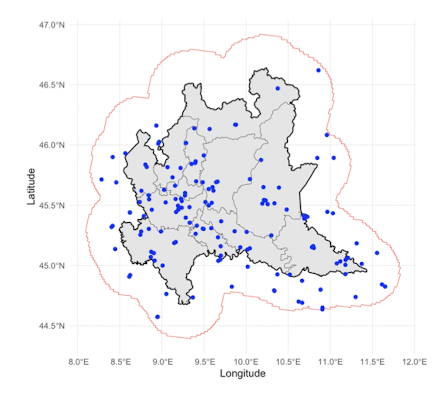
\includegraphics[width=\textwidth,height=\textheight,keepaspectratio]{Images/Zenodo/Agrimonia-dataset.png}
    \caption{Location of the stations in the Lombardy}
    \label{fig:mapLombardy}
\end{figure}
It exists also an upgraded version of this dataset named AGC (Agrimonia grid covariates) and it's a equidistant grid of 0.1° x 0.1° across the Lombardy region.
\begin{figure} [h]
    \centering
   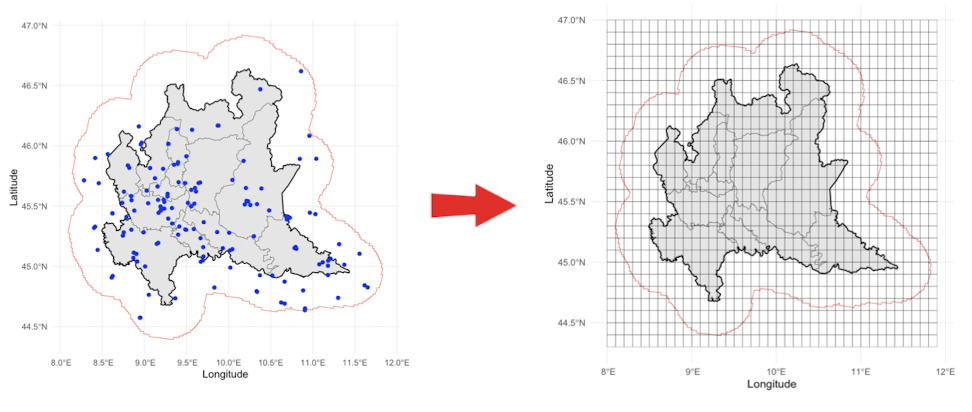
\includegraphics[width=\textwidth,height=\textheight,keepaspectratio]{Images/Zenodo/AGC.png}
    \caption{Location of the stations in the Lombardy}
    \label{fig:mapLombardy}
\end{figure}
\subsection{Methodologies}
The programming language used is mostly python and the main libraries used are: pandas, numpy, tensor flow and sk learn.
\\The models created are as follows:
\begin{itemize}
    \item Linear regression
    \item Regression with neural networks
    \item Recurrent neural network (RNN)
    \item Long short-term memory networks (LSTM networks)
    \item Convolutional neural network (CNN)
\end{itemize}
The estimator that were considered are mae (mean absolute error) and mse (mean squared error). The results are as follows:
\begin{table}[!ht]
    \centering
    \begin{tabular}{|l|l|l|l|l|l|l|l|l|l|}
    \hline
        \textbf{Tipe of regressio}n & \textbf{r2} & \textbf{mae} \\ \hline
        Linear regression & 0.46 & 10.76 \\ \hline
        Regression with neural networks & 0.70 & 146.72 \\ \hline
        RNN & 0.0067 & 15.95 \\ \hline
        LSTM networks & -7.15 & 8.79 \\ \hline
        CNN & -1324.27 & 397572.56 \\ \hline
  
    \end{tabular}
\end{table}
\\\underline{Note:} The station considered at this stage is the station Bertonico Via Moro (station id: 1266).

\subsection{Creating a subset for the dataset}
From here until the end of this thesis, only stations measuring the variable '$AQ\textunderscore\text{nh}{3}$' (i.e., stations measuring ammonia) were selected and used, totaling 10. Next, the station with the parameter 'IDStations' equal to 1266 was used. 
Note: For all types of regression, all variables in the dataset were used as regressors, except: 'IDStations', 'Latitude', 'Longitude', 'Time', 'Altitude' and '$AQ\textunderscore\text{PM}{25}$'.
\\The response variable is PM10. It represents the particulate matter with a diameter of 10 micrometers or less. It is a type of air pollutant consisting of solid particles and liquid droplets suspended in the air. These particles can originate from various sources, including dust, smoke, pollen, and emissions from vehicles, industrial processes, and construction activities.

\subsection{Pre processing of the data}
Before starting with all the procedures it was necessary to modify the dataset for speeding up the convergence of algorithms.
\\After selecting the features of interest it was necessary to scale the data using MinMax scaling.
\\As regards data splitting, a 67\% subdivision was made for the training set and 33\% for the test set.
\\Furthermore, as regards the algorithms based on neural networks, 100 epochs and batch size equal to 1 were made.

\subsection{Linear regression}
Classical regression was used, furthermore both x and y were divided into train set and test set with a 70-30 split (70$\%$ train and 30$\%$ test).
\subsection{Neural network design}
For this type of regression the neural network model is as follows:
\\As you can see from the image there are 4 layers of 32 neurons each. The activation function is the relu. The number of epochs is 100.
\\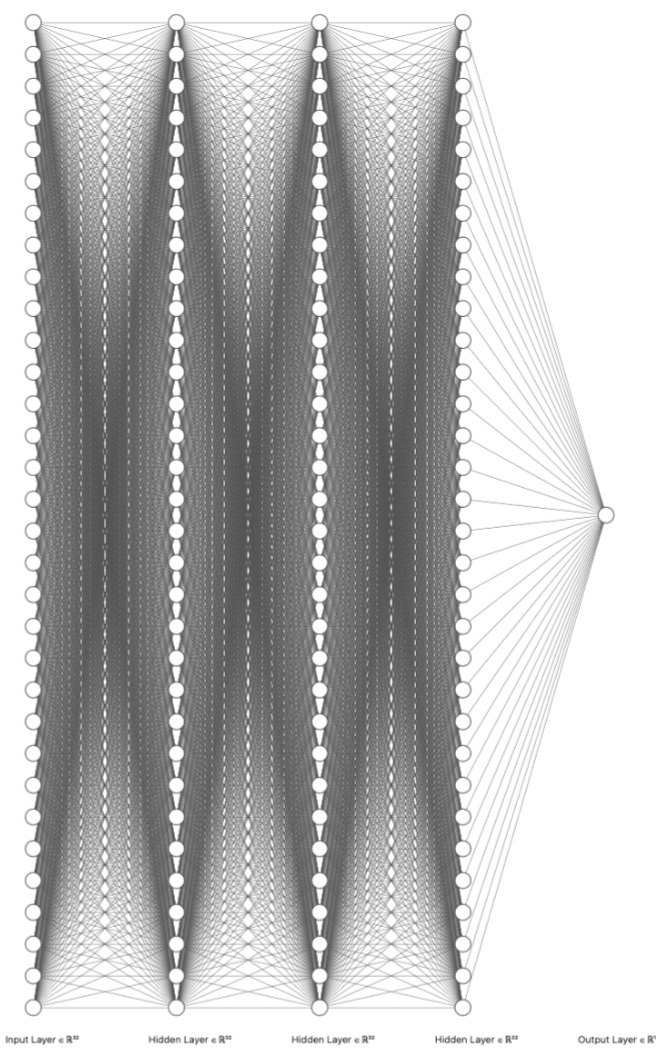
\includegraphics[scale = 0.75]{Images/NnStructure.png}
\subsection{Recurrent neural network (RNN)}
To improve performance, the data was first normalized before being used within the model.
\\The number of epochs is 100.

\subsection{Long short term memory networks (LSTM)}
Both x's and y's were split into train sets and test sets with a 70-30 split (70\% train and 30\% test).
The model consists of the following layers:
\\An LSTM layer with 50 neurons, a ReLU activation function, and an input shape of (1, X\_train.shape[2]). This means that the model expects input sequences of length 1, with X\_train.shape[2] functionality in each time step. The LSTM level can learn to extract useful functions from the input sequence and acquire time dependencies.
\\A dense output layer with a single neuron and no activation function (meaning it will produce a continuous value).
\\The Adam optimizer was used. The number of epochs is 100.

\subsection{Results}
\subsubsection{Cross-validation}
The results for the cross-validation are the one in the table ~\ref{tab:tableeee5}.

\begin{table}[!ht]
    \centering
    \begin{tabular}{|l|l|l|l|l|l|l|}
    \hline
        Type of regression & r2 & ~ & rmse & ~ & mae & ~ \\ \hline
        ~ & training  & test & training & test & training & test \\ \hline
        Linear regression & 0.51 & 0.54 & 13.20 & 14.15 & 9.47 & 10.34 \\ \hline
        Neural networks & 0.729 & 0.622 & 9,837 & 12,884 & 6,650 & 8,935 \\ \hline
        RNN & 0.5411 & 0.55 & 12.76 & 13.89 & 8.9 & 9.00 \\ \hline
        LSTM  & 0.756 & 0.659 & 9.32 & 12.22 & 6.45 & 8.63 \\ \hline
    \end{tabular}
    \label{tab:tableeee5}
    \caption{Regression performace of cross-validation}
\end{table}

\subsection{K-fold}
For all the following examples was used a crossvalidation kfold with k = 5.
\\The results are shown in table ~\ref{tab:table}.
\begin{sidewaystable}
    \centering
    \begin{tabular}{|l|l|l|l|l|l|l|l|}
    \hline
        Tipo di regressione utilizzata & r2 & & rmse &&  mae & variance  & \\ \hline
         & training & test & training & test & training & test & training \\ \hline
        Regressione lineare & 0.5355 & -0.193 & 13.18 & 17.36 & 9.53 & 13.19 & 174.18 \\ \hline
        Regressione con neural network & -107424.06 & -346555.80 & 3460.70 & 3626.38 & 3082.85 & 3261.72 & 8.99e+06 \\ \hline
        RNN & 0.62 & 0.069 & 11.87 & 16.95 & 7.91 & 12.09 & 140.84 \\ \hline
        LSTM networks & -1163.72 & -903.49 & 499.13 & 495.75 & 421.45 & 414.13 & 120511.51 \\ \hline
    \end{tabular}
    \caption{Regression performance of kFold }
    \label{tab:table}
\end{sidewaystable}



\subsection{Graphical comparison}
\subsection{}